%%%%%%%%%%%%%%%%%%%%%%%%%%%%%%%%%%%%%%%%%%%%%%%%%%%%%%%%%%%%%%%%%%%%%%%
%%%%%%%%%%%%%%%%%%%%%%%%%%%%%%%%%%%%%%%%%%%%%%%%%%%%%%%%%%%%%%%%%%%%%%%
%%%%%                                                                 %
%%%%%     <file_name>.tex                                             %
%%%%%                                                                 %
%%%%% Author:      <author>                                           %
%%%%% Created:     <date>                                             %
%%%%% Description: <description>                                      %
%%%%%                                                                 %
%%%%%%%%%%%%%%%%%%%%%%%%%%%%%%%%%%%%%%%%%%%%%%%%%%%%%%%%%%%%%%%%%%%%%%%
%%%%%%%%%%%%%%%%%%%%%%%%%%%%%%%%%%%%%%%%%%%%%%%%%%%%%%%%%%%%%%%%%%%%%%%

\chapter{Task Description}
%\phantomsection\addcontentsline{toc}{chapter}{Task Description 2}
%\markboth{Task Descrition}{Task Description 2}
This appendix presents in the following pages the initial task description. 

\begin{figure}[h!]
  \centering \includegraphics[width=0.55\textwidth]{content/task.pdf}
 \end{figure}

\includepdf[pages={2-}, pagecommand={\thispagestyle{headings}}, turn=false, scale=0.9]{content/task.pdf} % addtotoc={9, {appendix}, 0, {Task}, {task}}

\chapter{Declaration of Authorship}

%
\includepdf[pagecommand={\thispagestyle{headings}}, turn=false, scale=0.9]{includes/plagiarism_scanned.pdf}
%Include the declaration of authorship (\url{http://www.ethz.ch/faculty/exams/plagiarism/}) with the \shell{\textbackslash includepdf} command
%(sign it and scan it).
% include the signed declaration of authorship!
%\includepdf[pages=-, turn=false, scale=0.9]{... .pdf}


\chapter{File Structure}
\label{chapt:files}
\addtocounter{table}{1}
\addcontentsline{lot}{section}{\Alph{chapter}.\arabic{table}.\hspace{1pt} Directory and File Tree}
The following chapter gives an overview of all project files and a guidance how to program an adequate C or Assembler program, how to use the OpenRISC tool chain, how to generate Stimuli and Expected Responses and how to simulate. Table \Alph{chapter}.\arabic{table}. shows the directory tree of the main project folder \textit{./or10n/}.

\begin{center}
Table \Alph{chapter}.\arabic{table}.: Directory and File Tree
\end{center}
\begin{flushleft}
\dirtree{%
.1 ./or10n/.
  .2 README \DTcomment{Some general information about the project}.
  .2 cockpit.log \DTcomment{umcL180 Cockpit Log File}.
  .2 calibre \DTcomment{MentorGraphics' Calibre folder}.
    .3 drc \DTcomment{Design Rule Check}.
      .4 *.drc* \DTcomment{DRC reports}.
    .3 lvs \DTcomment{Layout versus Schematic}. 
      .4 chip.lvs.report \DTcomment{LVS Report}.
      .4 chip.lvs.report.ext \DTcomment{Circuit Extraction Report}.
      .4 verilog2spice \DTcomment{Verilog to Spice Conversion Scripts}.
  .2 docs \DTcomment{Documentations}.
    .3 task.pdf \DTcomment{Task Description}.
    .3 umcL180\_*\_rule.pdf \DTcomment{Design and Layout rules of umcL180}.
    .3 comparison \DTcomment{Comparison between architectures}.
      .4 ArchitectureComparison.csv \DTcomment{Table with Data}.
      .4 area\_*.txt \DTcomment{Area Reports}.
      .4 comp.m \DTcomment{Matlab Script to generate Comparison Diagram}.
      .4 comp\_table.csv \DTcomment{Table with MOPS for comp.m}.
      .4 results.png \DTcomment{Comparison Diagram}.
      .4 timing\_*.txt \DTcomment{Timing Reports}.
    .3 presentation \DTcomment{Presentation files}.
      .4 * \DTcomment{TODO TODO TODO}.
    .3 report \DTcomment{Report Files}.
      .4 Makefile \DTcomment{Makefile for Report Files}.
      .4 README \DTcomment{Some Comments about the Report}.
      .4 report.pdf \DTcomment{Final Report File}.
      .4 report.tex \DTcomment{Main $\LaTeX$ File}.
      .4 content \DTcomment{All $\LaTeX$ Content Files}.
      .4 figures \DTcomment{All included Figures}.
    .3 schematics \DTcomment{Schematics of the Project}.
  .2 encounter \DTcomment{Cadence's Encounter Files}.
    .3 reports \DTcomment{TODO TODO TODO}.
  .2 modelsim \DTcomment{Mentor Graphics' ModelSim Files}.
    .3 gate \DTcomment{Gate-Level Working Folder}.
    .3 reports  \DTcomment{IPC reports}.
    .3 scripts  \DTcomment{Scripts}.
      .4 compile.do  \DTcomment{Normal Compile Script}.
      .4 compile\_gate.sh  \DTcomment{Gate-Level Compile Script}.
      .4 sim\_postlayout.sh  \DTcomment{Start Script for Gate-Level Simulation}.
      .4 *.do  \DTcomment{ModelSim Wave Files}.
      .4 work  \DTcomment{Main Working Folder}.
    .3 vcd  \DTcomment{VCD Files}.
    .3 modelsim.ini  \DTcomment{Library Paths}.
  .2 setup \DTcomment{Setup Scripts}.
    .3 setup.csh \DTcomment{Setup Script}.
  .2 simvectors \DTcomment{Simulation vectors}.
    .3 * \DTcomment{Programs}.
      .4 exp.txt \DTcomment{Expected Responses File}.
      .4 stim.txt \DTcomment{Stimuli File}.
    .3 misses \DTcomment{Miss Files}.
      .4 dataMiss.txt \DTcomment{Data Memory Miss File}.
      .4 instrMiss.txt \DTcomment{Instruction Memory Miss File}.
  .2 sourcecode \DTcomment{Source Code}.
    .3 includes \DTcomment{Include Files}.
      .4 defines.sv \DTcomment{Definition File}.
    .3 alu.sv \DTcomment{Arithmetic Logic Unit}.
    .3 chip.sv \DTcomment{Chip Entity}.
    .3 controller.sv  \DTcomment{Controller}.
    .3 cpu.sv \DTcomment{CPU}.
    .3 data\_mem.sv \DTcomment{Data Memory}.
    .3 instr\_mem.sv \DTcomment{Instruction Memory}.
    .3 monitor.sv \DTcomment{Covergroup Monitor}.
    .3 mult.sv \DTcomment{Multiplier}.
    .3 registers.sv \DTcomment{General-Purpose Registers}.
    .3 sp\_registers.sv \DTcomment{Special-Purpose Registers}.
    .3 SY180\_*\_wrapper.vhd \DTcomment{Memory Wrapper}.
    .3 tb.sv \DTcomment{Testbench for Normal Simulation}.
    .3 tb\_chip.sv \DTcomment{Testbench for Gate-Level Simulation}.
    .3 top.sv \DTcomment{Top Entity}.
  .2 sw \DTcomment{Software to run on OR10N}.
    .3 bin2stim \DTcomment{Script to generate Stimuli from Binary File}.
      .4 bin2stim \DTcomment{Executable of bin2stim.}.
      .4 bin2stim.c \DTcomment{Source Code}.
    .3 libs \DTcomment{TODO TODO TODO}.
    .3 mul2muld \DTcomment{Scripts which inserts Double-word multiplication}.
      .4 mul2muld \DTcomment{Executable of mul2muld}.
      .4 muld2muld.c \DTcomment{Source Code}.
    .3 ref \DTcomment{Reference Files}.
      .4 common.mk \DTcomment{Makefile of the OpenRISC Tool Chain}.
      .4 cr0.* \DTcomment{Assembler Macros}.
      .4 link.ld \DTcomment{Linker File}.
    .3 testscripts \DTcomment{Assembler Scripts}.
      .4 *.S \DTcomment{Assembler Programs}.
    .3 *.bin \DTcomment{Binary Files}.
    .3 *.exe \DTcomment{Executables}.
    .3 *.read \DTcomment{Readable Binary File TODO}.
    .3 *.c \DTcomment{Source Codes}.
    .3 *.h \DTcomment{Header Files}.
    .3 Makefile \DTcomment{Makefile of the OpenRISC Tool Chain}.
  .2 synopsys \DTcomment{Synopsys Files}.
    .3 * \DTcomment{TODO TODO TODO}.
  .2 tetramax \DTcomment{Synopsys' TetraMAX Files}.
    .3 * \DTcomment{TODO TODO TODO}.
}
\end{flushleft}

\section{Assembler Coding}

\section{Stimuli Generation from Assembler programs}

\section{C programing}
- Linker File\\
- Memory Addressig\\
- qprint\\ \\
- make
\section{Stimuli Generation from C programs}

\section{RTL simulation}
For compilation of the \gls{rtl} model use the following script.

\begin{shellenv}
cd ./modelsim/
./scripts/compile.do
\end{shellenv}

After this step you can start ModelSim with appropriate parameters:

\begin{shellenv}
vsim-10.2a -lib work -voptargs=+acc [-GPROG=default ...] tb &
\end{shellenv}

Table \ref{tab:param} gives an overview of the most important parameters. If you want to do some coverage analyse use \shell{-coverage} this starts ModelSim in coverage mode where you can check code coverage and covergroups for the chosen program after simulation.

\begin{savenotes}
\begin{table}[htbp]
 \caption{Parameter for Simulation}
 \label{tab:param}
 \centering\begin{tabular}{|l|p{2cm}|r|p{8cm}|} \hline
param & example & default & Explanation \\ \hline
-coverage & &  & Start simulation in coverage mode. \\ \hline
-GPROG= & matrixMul, ... & default & Program which should be simulated \\ \hline
-GMODE= & default, \newline file & default & Misses are generated pseudo-randomly \newline Misses are read from Miss Files.\footnote{Misses are read cycle by cycle from the DataMiss.txt and InstrMiss.txt files which can be found and edited in the /or10n/simvectors/ folder.} \\ \hline
-GIMISS= & 15, ... & 5 & Propability of an instruction miss. (def. mode) \\ \hline
-GIMISS= & 90, ... & 33 & Propability of a data miss. (default mode) \\ \hline
-GRUNS= & 10, ... & 1 & Numbers of runs to be executed (default mode) \\ \hline
\end{tabular}
\end{table}
\end{savenotes}


\section{Gate-Level simulation}
dito


%\chapter{Datasets}
%If you have a data set comprising several test images, you could
%depict and describe them here. Use a simple naming scheme such that
%you can easily refer to certain elements of this data set in the text.


%\chapter{More Evaluation Results}
%If you conducted an extensive evaluation you could move surplus
%graphs/results to the appendix.


%\chapter{Algorithms / Tables}
%Large algorithm boxes and tables may clutter your chapters and impair
%the readability. If they are not very important, consider moving them
%to the appendix as well.


\chapter{ASIC Datasheet ($<$OR10N$>$)}

OR10N is an \gls{asic} implementation of the OpenRISC architecture which was designed by Matthias Baer and Renzo Andri as a Semester Thesis at the \gls{iis} at ETH Zurich. 


\minitoc 

\section{Features}
\begin{itemize}
\item OpenRISC 1200 32-Bit architecture.
\item 72 \gls{orbis} instructions. (see Table \ref{tab:instr} and \ref{tab:instr_det})
\item Additional instruction for End of Computation. (l.cust1)
\item 33-bit signed (hardware) multiplier.
\item Debugging interface. Messages can be printed character-wise on Data Output.
\item Test interface for cache misses.
\item Full Scan-Chain (Flaw detection)
\end{itemize}

%\section{Applications}


%\section{Description}


\section{Packaging}
Package QFN56 is used with 16 power pins and 40 user pins.

\section{Bonding Diagram}
The 16 power pins and the clock pin are arranged the same way as it is on the  Standard QFN56 tester board. See figures \ref{fig:bonding} and \ref{fig:pinout2} for more details. Pin 4-6 and 9-13 (\textit{Data\_DIO}) are bidirectional.
\begin{figure}[htbp]

  \centering \includegraphics[width=0.9\textwidth]{./figures/qfn56_180_std}
  \caption{Bonding diagram.}
\label{fig:bonding}
\end{figure}
\clearpage
\section{Pin Map}

\begin{figure}[!htbp]

  \centering \includegraphics[width=1.0\textwidth]{./figures/asic_pinout}
  \caption{$<$OR10N$>$ pinout.}
  \label{fig:pinout2}
\end{figure}
\begin{landscape}
\section{Pin Description}
Table \ref{tab:pins} describes pin usage. The first four are power pins, followed by the user-defined pins.
%\begin{table}[!tbph]
% \caption{Power Pins}
%% \label{tab:power_pins}
% \centering\begin{tabular}{|r| l| l|} \hline
%14; 28; 42; 56 & gnd\_p & Pad Ground \\ \hline
%01; 15; 29; 43 & vcc\_p & Pad Supply \\ \hline
%%07; 21; 35; 49 & gnd\_c & Core Ground \\ \hline
%08; 22; 36; 50 & vcc\_c & Core Supply \\ \hline
% \end{tabular}

%\end{table}

\begin{savenotes}
\begin{table}[htbp]
 \caption{Pin Description. (Power, IO, Clock, Reset, Test)}
 \label{tab:pins}
 \centering\begin{tabular}{|r| p{3cm}|p{3cm} |p{3cm} |p{3cm}|p{3cm}|} \hline
No. & Name & Setup &Run & Readout & Test \\ \hline

14; 28; 42; 56 & gnd\_p & \multicolumn{4}{l|}{Pad Ground} \\ \hline
01; 15; 29; 43 & vcc\_p & \multicolumn{4}{l|}{Pad Supply} \\ \hline
07; 21; 35; 49 & gnd\_c & \multicolumn{4}{l|}{Core Ground} \\ \hline
08; 22; 36; 50 & vcc\_c & \multicolumn{4}{l|}{Core Supply} \\ \hline
2-3 & Mode\_SI & \multicolumn{4}{ l| }{Defines Mode. See \ref{sec:mode} for further information.} \\ \hline
4-6; 9-13 & Data\_DIO & Data Input to\newline memories & Debugging\newline Output (qprint) & Data Output\newline from memories & - \\ \hline
16-20; 23-27 & PC\_DO & - & \gls{pc} in \glslink{id}{ID} stage & - & Scan\_In\_TI \\ \hline
30-34;37-41 & Addr\_DI[9:0] & \multirow{4}{*}{Memory Address}  & - &\multirow{4}{*}{Memory Address} & Scan\_Out\_TO \\ 
44 & Addr\_DI[10] & & - & & - \\
45 & Addr\_DI[11] & & Instr\_Ack\_TI\footnote{If set to 0 a cache miss from the instruction memory will occur.} &  & - \\ 
46 & Addr\_DI[12] &  & Data\_Ack\_TI\footnote{If set to 0 a cache miss from the data memory will occur.}  &  & - \\ \hline
47 & Rst\_RBI & \multicolumn{4}{l|}{Reset signal. (Active low)} \\ \hline
48 & Clk\_CI & \multicolumn{4}{l|}{Clock Signal} \\ \hline
51 & Scan\_En\_TI &- &- &- & Scan Enable \\ \hline
52 & Test\_En\_TI &- &- &- & Test Enable \\ \hline
53 & Flag\_SO &- & Flag Signal &- &- \\ \hline
54 & Stall\_SO &- & Stall Signal &- &- \\ \hline
55 & Eoc\_SO &- & End of Computation signal &- &- \\ \hline
 \end{tabular}
\end{table}
\end{savenotes}
\end{landscape}
 
%\section{Interface Description}


%\section{Register Map}

\section{Memory Addressing}
\label{sec:mem_addr}
Data can be written or read bytewise from chip. Internally, data is stored wordwise (4 Bytes). The memory addressing scheme is illustrated in Table \ref{tab:addr_scheme} and table \ref{tab:byteorder} shows the byte addressing. 
\begin{table}[htbp]
 \caption{Address scheme}
 \label{tab:addr_scheme}
\centering\begin{tabular}{|l| l|} \hline
 \multirow{2}{*}{Addr\_DI[12]} & 0 points to the instruction memory \\ 
                               & 1 points to the data memory \\ \hline
 Addr\_DI[11:2] & word address \\ \hline
 Addr\_DI[1:0] & byte address \\ \hline

 \end{tabular}
\end{table}

\begin{table}[htbp]
 \caption[Bit and Byte Ordering]{Bit and Byte Ordering \cite{or1000}}
 \label{tab:byteorder}
\centering\begin{tabular}{|c c|c c|c c|c c|} \hline
 Bit 31 & Bit 24 & Bit 23 & Bit 16 & Bit 15 & Bit 8 & Bit 7 & Bit 0 \\ \hline
\multicolumn{2}{|c|}{MSB} & & & & & \multicolumn{2}{c|}{LSB} \\ \hline
\multicolumn{2}{|c|}{Byte Address 00} & \multicolumn{2}{c|}{Byte Address 01} & \multicolumn{2}{c|}{Byte Address 10} & \multicolumn{2}{c|}{Byte Address 11} \\ \hline 

 \end{tabular}
\end{table}

Table \ref{tab:mem_map} shows all cpu-side relevant addresses and their usage. For registers which are specially used by the compiler consider the OpenRISC 1000 Architecture Manual (\cite{or1000}, Ch. 16.2).
\begin{table}[htbp]
 \caption{Special Memory Mapping}
 \label{tab:mem_map}
\centering\begin{tabular}{|l|r|l|p{9cm}|} \hline
memory & address & name & usage \\ \hline
data & 0x1FFF & std\_out & Bytes written to this address are mapped to the output \textit{Data\_DIO}. (qprint) \\ \hline
\gls{gpr} & (r9) 0x9 & LR & Link address used for l.jal(r) \\ \hline
\gls{spr} & 0x11 & SR & The Supervision Register contains branch, carry and overflow flags. \\
$\rightarrow$SR & 0x9 & F & (Branch) Flag \\
$\rightarrow$SR & 0xA & CY & Carry Bit \\
$\rightarrow$SR & 0xB & OV & Overflow Bit \\ \hline
\gls{spr} & 0x2801 & MACLO & Contains lower 32 bits of l.muld(u) operations. \\ \hline
\gls{spr} & 0x2802 & MACHI & Contains higher 32 bits of l.muld(u) operations. \\ \hline

 \end{tabular}
\end{table}



\clearpage

\section{Operation Modes}
\label{sec:mode}
OR10N runs in 4 different operational modes and 1 test mode. Table \ref{tab:pins} shows pin usage for all functional modes separately.
\subsection{Functional Modes}
\subsubsection{IDLE}
CPU is in IDLE mode if Mode\_SI[1:0] is set to 00.\\
CPU is disabled, memories are not written. The chip drives the bidirectional signal Data\_DIO to all zero.
\subsubsection{SETUP}  
CPU is in SETUP state if Mode\_SI[1:0] is set to 10.\\
In this mode the data can be written from outside to both of the memories. Data is laid bytewise to the bidirectional pin Data\_DIO and is saved at address Addr\_DI on rising edge.  Section \ref{sec:mem_addr} explains how the bytes are addressed.
\subsubsection{RUN}
CPU is in RUN mode if Mode\_SI[1:0] is set to 01.\\
Main Mode. CPU runs until end of computation is reached. (special instruction l.cust1), then signal Eoc\_SO is set to 1. During RUN state some outputs can be used for debugging.
\begin{itemize}
\item PC\_DO: Current \gls{pc} in \gls{id} stage.
\item Data\_DIO: Is either 0 or an ASCII character. Can be printed out using qprint (C programs) or writing to address 0x1FFF (Assembler).
\item Flag\_SO: Current Flag.
\item Stall\_SO: Indicates whether there is a stall at this time. 
\item Eoc\_SO: Indicates that the end of the program were reached.
\end{itemize}

Although no misses can occur on this chip, there is a possibility to inject a delibarate miss to check cpu's ability for handling them. The following inputs are used for this option.
\begin {itemize}
\item Addr\_DI[11]=Instr\_Ack\_TI: If this signal is set to 0, the instruction memory will cause a miss in the next cycle.
\item Addr\_DI[12]=Data\_Ack\_TI: If this signal is set to 0, the data memory will cause a miss in the next cycle.
\end{itemize}

\subsubsection{READOUT}
CPU is in RUN mode if Mode\_SI[1:0] is set to 11.\\
In the READOUT mode both memories can be read out using the address scheme from section \ref{sec:mem_addr}. The byte at address Addr\_DI is read from memory and put on Data\_DIO with one latency. 

\subsection{Test Modes}
If Test\_En\_TI is set to 1 both memory macrocells are bypassed. This allows a better test coverage using ATPG. See schema TODO for more information.

\section{Timing}
OR10N is time-optimized for register to register allowing for a clock period of 2.75 ns (364 MHz) in RUN mode. If debugging outputs or qprint is used longest path lengthens to 4.14 ns (241 MHz) or 6.04 ns (165 MHz), respectively. Fig. \ref{fig:timing} and Table \ref{tab:timing} illustrate timing the maximum clocking frequency. As can be seen on Figure \ref{fig:timing} there is one in-to-out path: From mode input (\textit{Mode\_SI}) to data output (\textit{Mode\_DIO}). This leads not to a conflict with the clock period $T_{SETUP}$, $T_{RUN}$ or $T_{READOUT}$.\footnote{If the order SETUP-RUN-READOUT is not violated, there is at least one latency until inputs affect outputs such that the longer path does not matter.}

\begin{figure}[htbp]
  \centering
  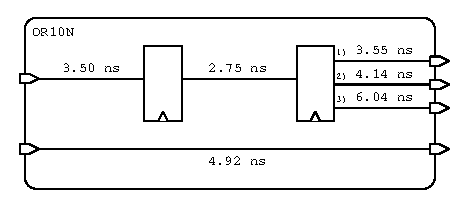
\includegraphics[width=0.7\linewidth]{./figures/delays}
  \caption[Timing diagram]{Timing diagram.\\1) w/o debugging, 2) debugging information, 3) debugging incl. qprint}
  \label{fig:timing}
\end{figure}
\begin{table}[htbp]
 \caption{Longest path and maximum frequency $\sim$ Mode}
 \label{tab:timing}
\centering\begin{tabular}{|l|r|r|} \hline
Mode & $t_{lp}$ & $f_{max}$ \\ \hline
SETUP & 3.50 ns & 285 MHz \\ \hline
RUN & 2.75 ns & 363 MHz \\ \hline
RUN+debug & 4.14 ns & 241 MHz \\ \hline
RUN+qprint & 6.04 ns & 165 MHz \\ \hline
READOUT & 3.55 ns & 282 MHz \\ \hline

 \end{tabular}
\end{table}


\section{Electrical Specifications}
\begin{table}[htbp]
 \caption[DC characteristics]{DC characteristics \cite{faraday}}
 \label{tab:elect_rec}
\centering\begin{tabular}{|l|l|r|r|c|} \hline
Symbol & Description & Min. & Max. & Unit \\ \hline
$V_{Il}$ & Input low voltage & - & 0.8 & $V$ \\ \hline
$V_{Ih}$ & Input high voltage & 2.0 & - & $V$ \\ \hline
$V_{Ol}$ & Output low voltage & - & 0.4 & $V$ \\ \hline
$V_{Oh}$ & Output high voltage & 2.4 & - & $V$ \\ \hline
$I_O$ & Output driving & \multicolumn{2}{r|}{8} & $mA$ \\ \hline

 \end{tabular}
\end{table}

\subsection{Recommended Operating Regions}
\begin{table}[htbp]
 \caption[Recommended Operating Conditions]{Recommended Operating Conditions \cite{faraday}}
 \label{tab:elect_rec}
\centering\begin{tabular}{|l|l|r|r|r|c|} \hline
Symbol & Description & Min. & Typ. & Max. & Unit \\ \hline
\textit{vcc\_c} & Core power supply & 1.62 & 1.8 & 1.98 & $V$ \\ \hline
\textit{vcc\_p} & Pad power supply & 2.97 & 3.3 & 3.63 & $V$ \\ \hline
$T_J$ & Operating junction temperature & -40 & 25 & 125 & $^{\circ} C$ \\ \hline

 \end{tabular}
\end{table}
\clearpage
\subsection{Absolute Maximum Ratings}
\begin{table}[ht]
 \caption[Absolute Maximum Ratings]{Absolute Maximum Ratings \cite{faraday}}
 \label{tab:elect_rec}
\centering\begin{tabular}{|l|l|c|c|} \hline
Symbol & Description & Rating & Unit \\ \hline
\textit{vcc\_c} & Core power supply & -0.5 $\sim$ 2.5 & $V$ \\ \hline
\textit{vcc\_p} & Pad power suplly & -0.5 $\sim$ 4.6 & $V$ \\ \hline
$V_{In}$ & Input voltage &  -0.5 $\sim$ 4.6 & $V$ \\ \hline
$I_{In}$ & DC input current & 50 & $mA$ \\ \hline
$I_{Out}$ & DC output current & 50 & $mA$ \\ \hline
 \end{tabular}
\end{table}
